\chapter{Работа с очередями FIFO}

\emph{Интерфес FIFO. Асинхронных режим. Режимы работы FIFO: Standard и First Word Fall Through. Интерфейс AXI Stream.}

\section{Содержание главы}

Основной литературой по FIFO является PG057. Требуется:
\begin{itemize}
\item описать всю последовательность действий по созданию и кастомизации ядра FIFO, а также включению его в код на VHDL, сделав при этом упор на интерфейс \emph{Native} и на интерфейс \emph{AXI4-Stream} (про интерфейс AXI4 Memory Mapped достаточно упомянуть);
\item написать testbench для ядра FIFO, чтобы показать его функциональность (т.е. то, как ядро работает), привести пример временных форм сигналов из симулятора;
\item описать принцип работы FIFO (описать два указателя~-- на начало и конец очереди в памяти, когда и как они увеличиваются и т.д.);
\item написать, отладить и описать VHDL-код усредняющего FIFO. Обязателен testbench.
\end{itemize}

\section{Что такое FIFO? VHDL-код FIFO на основе \\ регистров.}

\begin{figure}[h]
\centering
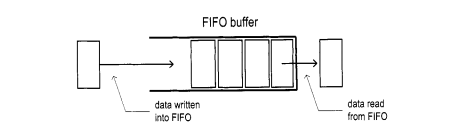
\includegraphics[width=0.6\textwidth]{fifo_bufer}
\caption{Концептуальная схема буфера FIFO}
\label{fifo_bufer_label}
\end{figure}

Буфер FIFO (first-in-first-out) является «эластичным» хранилищем между двумя подсистемами, как показано на концептуальной диаграмме рисунка 1.1.  Он имеет два управляющих сигнала, wr и rd, для операций записи и чтения. Когда утверждается wr, входные данные записываются в буфер. Операция чтения несколько вводит в заблуждение. Голова буфера FIFO всегда доступна и, следовательно, может быть прочитана в любое время. На самом деле сигнал rd действует как сигнал «удалить». Когда это утверждается, первый элемент (то есть голова) буфера FIFO удаляется, и становится доступным следующий элемент. Буфер FIFO является критическим компонентом во многих приложениях, и оптимизированная реализация может быть довольно сложной. В этом подразделе мы вводим простые,  кольцевые рисунки на основе циклических очередей.

\subsection{Реализация на основе циклических очередей}
Одним из способов реализации буфера FIFO является добавление схемы управления к регистровому файлу. Регистры в регистровом файле располагаются в виде круговой очереди с двумя указателями. Указатель записи указывает на начало очереди, а указатель чтения указывает на хвост очереди. Указатель продвигает одну позицию для каждой операции записи или чтения. Операция кольцевой очереди из восьми слов показана на рисунке 1.2.
	Буфер FIFO обычно содержит два сигнала состояния, полный и пустой, чтобы указать, что FIFO заполнен (т.е. не может быть записан) и пуст (т.е. не может быть прочитан) соответственно. Одно из двух условий возникает, когда указатель чтения равен указателю записи, как показано на рис. 1.2 (a), (f) и (i). Самая сложная задача разработки контроллера - получить механизм, позволяющий отличать два условия. Одна из схем заключается в использовании двух FFs для отслеживания пустых и полных статусов. FFs устанавливаются в '1' и '0' во время инициализации системы, а затем изменяются в каждом такте в соответствии со значениями wr и rd сигналов. Код показан в ниже:

\begin{figure}[h]
\centering
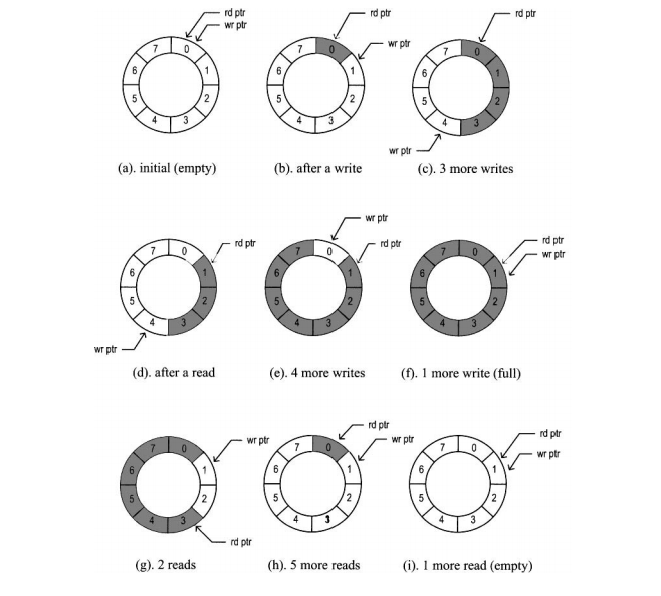
\includegraphics[width=1.1\textwidth]{circular_queue}
\caption{Буфер FIFO, основанный на кольцевой очереди.}
\label{circular_queue_label}
\end{figure}

\begin{Code}
\begin{lstlisting}

library ieee;
use ieee.std_logic_vector_1164.all;
use ieee.numeric_std.all;
entity fifo is
	generic (
		B: natural := 8;  -- numbrer of bits
		W: natural:= 4 -- number of address bits
	);
port (
	clk, reset:  in std_logic;
	rd, wr:  in std_logic;
	w_data: in std_logic_vector (B-1 downto 0);
	empty, full: out std_logic;
	r_data: out std_logic_vector (B-1 downto 0)
	);
end fifo;

architecture arch of fifo is
	type reg_file_type is array (2**W-1 downto 0) of

\end{lstlisting}
\end{Code}

\section{Интерфейс FIFO}

Ядро FIFO (first-in first-out - первый вошел, первый вышел) генератора может использоваться в любом приложении, требующем упорядоченного
хранения и извлечения, что позволяет создавать высокопроизводительные и оптимизированные по площади проекты.
Ядро обеспечивает оптимизированное решение для всех конфигураций FIFO и  максимальную производительность (до 500 МГц) при использовании
минимальных ресурсов.

Это ядро поддерживает Native интерфейс, AXI Memory Mapped и AXI4-Stream interface.
Оно может быть настроено с использованием модификаторов IP Vivado в каталоге
IP как завершенное решение с уже реализованной логикой управления, включая управление указателями
чтения и записи и генерацию флагов состояния.


\section{Оформление}

Очень хорошее и краткое введение в LaTeX можно найти в книге Столярова (\href{url}{http://www.stolyarov.info/books/latex3days/}).

\section{Заголовок 1-го уровня}
\subsection{Заголовок 2-го уровня}
\subsubsection{Заголовок 3-го уровня}

Текст. Текст. Текст. \emph{Текст курсивом.} Поставить тире~-- вот так. Текст в "<кавычках">.

Чтобы сделать новый абзац, нужно пропустить строку.

Пример кода:

\begin{Code}
\begin{lstlisting}
library IEEE;
use IEEE.STD_LOGIC_1164.ALL;

entity Latch is
    port ( C : in  STD_LOGIC;
           D : in  STD_LOGIC;
           Q : out STD_LOGIC);
end Latch;

architecture Behavioral of Latch is
    signal q_tmp : std_logic := '0';
begin
    latch_process: process (C, D)
    begin
        if (C = '1') then
            q_tmp <= D;
        end if;
    end process;
    Q <= q_tmp;
end Behavioral;
\end{lstlisting}
\end{Code}

Пример кода в строке: \lstinline?С = 1?. Или вот так: \lstinline?S(7 downto 1) <= S(6 downto 0);?. Здесь код помещен между знаками вопроса.

Пример нумерованного списка:

\begin{enumerate}
\item Пункт 1.
\item Пункт 2.
\item Пункт 3.
\end{enumerate}

Пример ненумерованного списка:

\begin{itemize}
\item Пункт 1.
\item Пункт 2.
\item Пункт 3.
\end{itemize}

Вот так оформляется таблица с тремя колонками:

\begin{table}[h]
\centering
\begin{tabular}{|c|c|c|}
\hline
input               & \multicolumn{2}{c|}{output} \\ \hline
r                   & code        & active         \\ \hline
\texttt{1{-}{-}{-}} & \texttt{11} & \texttt{1}     \\
\texttt{01{-}{-}}   & \texttt{10} & \texttt{1}     \\
\texttt{001-}       & \texttt{01} & \texttt{1}     \\
\texttt{0001}       & \texttt{00} & \texttt{1}     \\
\texttt{0000}       & \texttt{00} & \texttt{0}     \\
\hline
\end{tabular}
\end{table}

Рисование осуществляется с помощью пакета 'TikZ':

\begin{figure}[ht]
\centering
\begin{tikzpicture}[>=latex']
\tikzstyle{arith_op} = [draw, fill=blue!20, circle, minimum size=2em]

% inputs
\node at (0,4) (input_a) {\texttt{a}};
\node at (0,3) (input_b) {\texttt{b}};
\node at (0,1) (input_c) {\texttt{c}};
\node at (0,0) (input_1) {\texttt{1}};

% operations
\node[arith_op] at (1,3) (block_plus_1) {$+$};
\node[arith_op] at (1,1) (block_plus_2) {$+$};
\node[arith_op] at (2,2) (block_minus) {$-$};

% connections
\draw[->] (input_a) -- (1,4) -- node {} (block_plus_1);
\draw[->] (input_b) -- node {} (block_plus_1);
\draw[->] (input_c) -- node {} (block_plus_2);
\draw[->] (input_1) -- (1,0) -- node {} (block_plus_2);
\draw[->] (block_plus_1) -- (2,3) -- node {} (block_minus);
\draw[->] (block_plus_2) -- (2,1) -- node {} (block_minus);
\draw[->] (block_minus) -- (3,2);
\end{tikzpicture}
\caption{Оптимизированная комбинационная схема.}
\label{label_fig_1}
\end{figure}

Ссылка на рисунок делается по \emph{label} вот так: \ref{label_fig_1}.

Вставка скриншотов программ (PNG) возможна следующим образом (файл изображения находится в папке с кодом):

\begin{figure}[h]
\centering
\includegraphics[width=0.6\textwidth]{test_fig}
\caption{Некий рисунок}
\label{test_fig_label}
\end{figure}
